\documentclass[11pt]{article}

% ---------------------------------------------------------------------------
% OMNIS detailed documentation. Compiles with tectonic or any modern TeX.
% Author: Ansh Jain (github.com/ataylus). Team: Partly Everything.
% Theme: Palatino body, sans navy headings, navy accent, TikZ architecture.
% ---------------------------------------------------------------------------

\usepackage[T1]{fontenc}
\usepackage[utf8]{inputenc}
\usepackage[a4paper,margin=2.5cm]{geometry}
\usepackage{newpxtext}
\usepackage{newpxmath}
\usepackage{tgheros}            % sans family for headings
\usepackage[scaled=0.85]{beramono}
\usepackage{parskip}           % block paragraphs: no first-line indent, even spacing
\usepackage{microtype}
\usepackage{xcolor}
\usepackage{graphicx}
\graphicspath{{./}{../}}
\usepackage{float}             % [H] for exact placement, no floating/reordering
\usepackage{booktabs}
\usepackage{tabularx}
\usepackage{array}
\usepackage{enumitem}
\usepackage{titlesec}
\usepackage{fancyhdr}
\usepackage[most]{tcolorbox}
\usepackage{tikz}
\usetikzlibrary{positioning,arrows.meta,shapes.geometric,fit,backgrounds}
\usepackage[hidelinks]{hyperref}

% --- palette ---------------------------------------------------------------
\definecolor{navy}{RGB}{31,58,95}
\definecolor{navysoft}{RGB}{238,242,248}
\definecolor{ink}{RGB}{26,25,23}
\definecolor{muted}{RGB}{110,106,99}
\definecolor{line}{RGB}{205,201,193}
\definecolor{green}{RGB}{31,122,77}
\definecolor{amber}{RGB}{154,91,8}
\definecolor{red}{RGB}{179,38,30}
\definecolor{grey}{RGB}{95,107,122}

\hypersetup{colorlinks=true,linkcolor=navy,urlcolor=navy,citecolor=navy}
\color{ink}

% --- attribution -----------------------------------------------------------
\newcommand{\authorname}{Ansh Jain}
\newcommand{\authorhandle}{github.com/ataylus}
\newcommand{\watermark}{\authorname\,\textbar\,\authorhandle}

% --- headings in sans navy, thin rule under each section -------------------
\titleformat{\section}{\sffamily\bfseries\large\color{navy}}{\thesection}{0.7em}{}[{\color{line}\titlerule[0.5pt]}]
\titleformat{\subsection}{\sffamily\bfseries\normalsize\color{navy}}{\thesubsection}{0.6em}{}
\titlespacing*{\section}{0pt}{1.4em}{0.6em}
\titlespacing*{\subsection}{0pt}{1.0em}{0.35em}

% --- running header/footer (footer carries the watermark) ------------------
\pagestyle{fancy}
\fancyhf{}
\renewcommand{\headrulewidth}{0.3pt}
\renewcommand{\footrulewidth}{0.3pt}
\fancyhead[L]{\sffamily\footnotesize\color{muted}OMNIS}
\fancyhead[R]{\sffamily\footnotesize\color{muted}the partly omniscient auditor}
\fancyfoot[L]{\sffamily\footnotesize\color{muted}\watermark}
\fancyfoot[R]{\sffamily\footnotesize\color{muted}\thepage}

% --- helpers ---------------------------------------------------------------
\newcommand{\code}[1]{\texttt{\small #1}}
\newcommand{\chip}[2]{\textcolor{#1}{\sffamily\bfseries\footnotesize #2}}

\newtcolorbox{resultbox}{colback=navysoft,colframe=navy,boxrule=0.6pt,
  arc=2pt,left=10pt,right=10pt,top=8pt,bottom=8pt}
\newtcolorbox{findingbox}{colback=white,colframe=navy,boxrule=0.6pt,
  arc=2pt,left=10pt,right=10pt,top=8pt,bottom=8pt,
  borderline west={3pt}{0pt}{navy}}

% architecture node styles
\tikzset{
  io/.style={draw=muted,fill=white,rounded corners=2pt,font=\sffamily\scriptsize,
    align=center,inner sep=4pt,minimum height=8mm,text width=24mm},
  mod/.style={draw=navy,fill=navysoft,rounded corners=2pt,font=\sffamily\scriptsize\bfseries,
    text=navy,align=center,inner sep=4pt,minimum height=8mm,text width=24mm},
  outbox/.style={draw=green,fill=white,rounded corners=2pt,font=\sffamily\scriptsize,
    text=green,align=center,inner sep=4pt,minimum height=8mm,text width=24mm},
  side/.style={draw=muted,fill=white,dashed,rounded corners=2pt,
    font=\sffamily\scriptsize,align=center,inner sep=4pt,text width=24mm},
  flow/.style={-{Stealth[length=2mm]},draw=navy,thick},
  sideflow/.style={-{Stealth[length=2mm]},draw=muted,dashed},
}

\begin{document}

% ===========================================================================
% TITLE PAGE
% ===========================================================================
\begin{titlepage}
\thispagestyle{empty}
\begin{tikzpicture}[remember picture,overlay]
  \fill[navy] (current page.north west) rectangle ([yshift=-5.6cm]current page.north east);
  \node[anchor=west,text=white,font=\sffamily\bfseries\fontsize{40}{44}\selectfont]
    at ([xshift=2.5cm,yshift=-2.7cm]current page.north west) {O\,M\,N\,I\,S};
  \node[anchor=west,text=white,font=\itshape\Large]
    at ([xshift=2.55cm,yshift=-3.9cm]current page.north west) {the partly omniscient auditor};
  \node[anchor=west,text=navysoft,font=\sffamily\small]
    at ([xshift=2.55cm,yshift=-4.9cm]current page.north west)
    {Automated Compliance Evidence Collection \& Audit};
\end{tikzpicture}

\vspace*{5.9cm}

{\sffamily\bfseries\LARGE\color{navy} Detailed Documentation}\\[0.3em]
{\large Architecture, algorithms, results, and design decisions}

\vspace{0.9cm}

\noindent OMNIS reads security policies into requirements, links each requirement to
its evidence, tracks freshness and confidence, detects anomalies, and produces an
auditor-ready report with one honest number at the top. This document is the full
design writeup: how every stage works, what it measures, and why it was built this way.

\vspace{0.9cm}

\begin{tabular}{@{}p{3.6cm}l@{}}
\textbf{Problem statement} & PS3, Soci\'et\'e G\'en\'erale iHACK MYPLACE \\[3pt]
\textbf{Author} & \authorname\ (\authorhandle) \\[3pt]
\textbf{Team} & Partly Everything \\[3pt]
\textbf{Repository} & \url{https://github.com/ataylus/OMNIS} \\[3pt]
\textbf{Runtime} & Python 3.10+, offline, no API key required \\
\end{tabular}

\vspace{0.9cm}

{\sffamily\bfseries\color{navy}What is inside}\\[0.4em]
\begin{tabular}{@{}p{7.6cm}p{7.6cm}@{}}
\small The problem and the thesis & \small Results, measured \\
\small The architecture & \small The data and the integrity auditor \\
\small The algorithms: linking and scoring & \small Evidence collectors \\
\small The benchmark we audited & \small The dashboard and the report \\
\small The four edge cases & \small Design decisions and limitations \\
\end{tabular}\\[0.2em]
{\small\color{muted}Full contents on the next page.}

\vfill

\begin{resultbox}
\sffamily\small\color{ink}
\textbf{\color{navy}Three measured results.}
Detection precision \textbf{0.957} / recall \textbf{0.953} on the labelled bench.
Evidence linking recovers the correct requirement \textbf{54.7\%} of the time with the
ID hidden, against a \textbf{6.7\%} random baseline. The full pipeline runs
\textbf{500 requirements and 5,000 evidence records in under one second}. 102 tests pass.
\end{resultbox}

\vspace{0.3cm}
{\sffamily\footnotesize\color{muted}\watermark}
\end{titlepage}

% ===========================================================================
% CONTENTS
% ===========================================================================
\newpage
{\sffamily\bfseries\large\color{navy}Contents}
\vspace{0.4em}
{\color{line}\hrule height 0.5pt}
\vspace{0.6em}
\setcounter{tocdepth}{2}
\renewcommand{\contentsname}{\vspace{-2.2em}}
\tableofcontents

% ===========================================================================
\newpage
\section{Abstract}

A bank has to prove it follows its own rules. Not just follow them, prove it, to an
auditor who accepts nothing less than the receipt: the config file, the rotation log,
the access report. Those receipts are scattered across systems, and a compliance team
spends more than 72 hours per audit cycle hunting them down. A control can be working perfectly and
still fail the audit because nobody found the paperwork.

OMNIS reads the policies, links each requirement to its evidence, tracks how fresh that
evidence is, detects anomalies in the evidence corpus, and produces an auditor-ready
report with one honest number at the top: the Omniscience Index, a 0 to 100 measure of
how much the system actually knows and how much of that it trusts. The guiding idea is
that the system quantifies its own ignorance. A requirement with no evidence is reported
as \chip{grey}{UNKNOWN}, not quietly skipped. Evidence that matches nothing is left
unmapped, not forced.

Every number in this document is reproducible from the repository with a single command
and no network access.

% ===========================================================================
\section{The problem and the thesis}

The four edge cases the brief calls out, missing evidence, conflicting evidence,
low-confidence evidence, and ambiguity, are not corner cases bolted on at the end. They
are the centre of the problem. Real audit data is incomplete and contradictory, so a
tool that only works on clean data is useless. OMNIS treats imperfect data as the job.

Our thesis is honesty as a feature. Most compliance dashboards report a single green
number and hide the gaps. OMNIS does the opposite: it surfaces coverage, freshness, and
confidence separately, names every gap, and refuses to assert a link or a verdict the
data does not support. The headline test of this thesis came from the provided dataset
itself, described in Section~\ref{sec:finding}.

% ===========================================================================
\section{Architecture}

OMNIS is a modular monolith under the \code{omnis/} package. Each stage is a small,
testable module that passes typed domain objects to the next. There is no hidden state
and no service to stand up: the whole pipeline is a function from files to a report.

\begin{figure}[H]
\centering
\resizebox{\textwidth}{!}{%
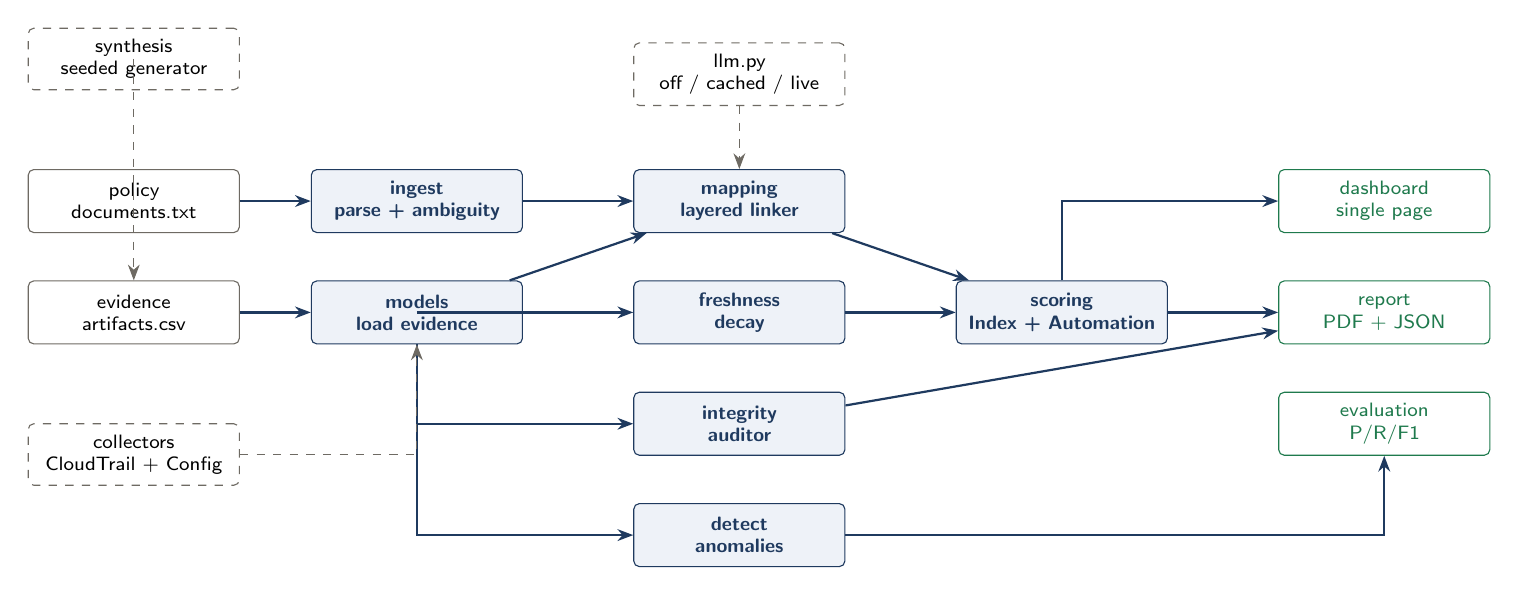
\begin{tikzpicture}[node distance=6mm and 9mm]
  \node[io] (pol) {policy\\documents.txt};
  \node[io,below=of pol] (ev) {evidence\\artifacts.csv};
  \node[side,below=10mm of ev] (col) {collectors\\CloudTrail + Config};
  \node[side,above=10mm of pol] (syn) {synthesis\\seeded generator};

  \node[mod,right=of pol] (ing) {ingest\\parse + ambiguity};
  \node[mod,right=of ev] (mod) {models\\load evidence};

  \node[mod,right=14mm of ing] (map) {mapping\\layered linker};
  \node[mod,below=of map] (fresh) {freshness\\decay};
  \node[mod,below=of fresh] (int) {integrity\\auditor};
  \node[mod,below=of int] (det) {detect\\anomalies};

  \node[mod,right=14mm of fresh] (score) {scoring\\Index + Automation};

  \node[outbox,right=14mm of score] (rep) {report\\PDF + JSON};
  \node[outbox,above=of rep] (dash) {dashboard\\single page};
  \node[outbox,below=of rep] (evalb) {evaluation\\P/R/F1};

  \node[side,above=8mm of map] (llm) {llm.py\\off / cached / live};

  \draw[flow] (pol) -- (ing);
  \draw[flow] (ev) -- (mod);
  \draw[flow] (ing) -- (map);
  \draw[flow] (mod) -- (map);
  \draw[flow] (mod) |- (fresh);
  \draw[flow] (mod) |- (int);
  \draw[flow] (mod) |- (det);
  \draw[flow] (map) -- (score);
  \draw[flow] (fresh) -- (score);
  \draw[flow] (score) -- (rep);
  \draw[flow] (score) |- (dash);
  \draw[flow] (det) -| (evalb);
  \draw[flow] (int) -- (rep);
  \draw[sideflow] (syn) -| (ev);
  \draw[sideflow] (col) -| (mod);
  \draw[sideflow] (llm) -- (map);
\end{tikzpicture}%
}
\caption{The pipeline. Solid arrows are the core data flow; dashed nodes are optional
inputs (synthetic data, mock collectors) and the dormant LLM adapter.}
\end{figure}

\begin{description}[leftmargin=0pt,style=nextline,itemsep=3pt,labelsep=0pt]
\item[\textcolor{navy}{ingest}] A deterministic structural parser. Reads the
  line-structured policy file into typed \code{Requirement} objects, tolerant of the
  messiness the sample actually contains (CRLF endings, a lowercase \code{scope:} field).
  It also flags ambiguous requirements at parse time (Section~\ref{sec:edge}).
\item[\textcolor{navy}{integrity}] An evidence-corpus auditor. Eight checks for the
  defect classes the data contains: duplicate descriptions, orphan references, impossible
  date orders, freshness that disagrees with the dates, status that contradicts confidence.
\item[\textcolor{navy}{mapping}] The layered linker (Section~\ref{sec:linking}).
\item[\textcolor{navy}{freshness}] A decay model (Section~\ref{sec:freshness}). Each
  requirement's audit frequency sets its staleness window; evidence loses weight as it ages
  past that window.
\item[\textcolor{navy}{scoring}] Per-requirement status and the headline roll-ups
  (Section~\ref{sec:scoring}).
\item[\textcolor{navy}{detect}] A transparent rule-based anomaly classifier for evidence
  records (Section~\ref{sec:detect}), targeting the five ground-truth classes.
\item[\textcolor{navy}{narrative}] An auditor-voice explanation for each verdict,
  template-driven by default with an optional LLM enrichment path.
\item[\textcolor{navy}{report}] The auditor-ready PDF and JSON (Section~\ref{sec:ui}).
\item[\textcolor{navy}{evaluation}] Precision, recall, and per-class F1 against the ground
  truth, plus the linking-accuracy metric.
\item[\textcolor{navy}{collectors}] Two mock integrations that pull evidence into the
  pipeline (Section~\ref{sec:collectors}).
\end{description}

% ===========================================================================
\section{The algorithms}

\subsection{Evidence linking}\label{sec:linking}

Linking each evidence record to a requirement runs in layers, stopping at the first
confident match. Every link carries the method that produced it and a confidence.

\begin{enumerate}[leftmargin=1.4em,itemsep=2pt]
\item \textbf{exact\_id}: the record's \code{requirement\_id} equals a known requirement.
  Confidence 1.0.
\item \textbf{framework\_rule}: a deterministic match on the record's framework and
  evidence type against the requirement's compliance mappings and evidence source.
\item \textbf{tfidf}: offline TF-IDF cosine similarity between the evidence text and the
  requirement text, above a similarity floor.
\item \textbf{unmapped}: nothing cleared the floor. The record is left unmapped, which is
  a reported finding, not an error.
\end{enumerate}

The TF-IDF layer is a small pure-Python implementation, so the linker runs offline with
no extra dependency. The similarity floor is set to 0.30 deliberately: evidence whose
text genuinely matches a requirement is linked, while generic or orphan-referencing
evidence is left unmapped rather than forced onto the nearest requirement. Leaving weak
evidence unmapped is the honest outcome and is exactly what the project's thesis demands.

\subsection{Freshness decay}\label{sec:freshness}

The brief names freshness a first-class feature, so it gets a model rather than a flat
cutoff. Each requirement carries an audit frequency, and that frequency sets how long its
evidence stays current:

\begin{center}
\sffamily\small
\begin{tabular}{@{}ll@{}}
\toprule
Audit frequency & Window (days) \\
\midrule
Daily, Continuous & 1 \\
Weekly & 7 \\
Monthly & 30 \\
Quarterly & 90 \\
Unknown (fallback) & 90 \\
\bottomrule
\end{tabular}
\end{center}

A record's freshness score decays exponentially, halving once per window:
\[
f \;=\; 0.5^{\,a / w},
\]
where $a$ is the record's age in days and $w$ is its audit-frequency window, which doubles
as the decay half-life. A brand-new record scores 1.0, one a full window old scores 0.5,
one three windows old scores about 0.125. A record whose age cannot be established scores
0.0, because an unverifiable age cannot be claimed as fresh. A record older than its window
without a fresh approval is reported stale.

One detail matters for trust. The age comes from the record's \code{freshness\_days} field,
not from subtracting dates, because the integrity auditor found the date columns internally
inconsistent on 455 of 500 sample rows. Freshness is computed against a fixed reference date
(2026-04-15), never wall-clock time, so every run and every test is reproducible.

\subsection{Compliance scoring and the Omniscience Index}\label{sec:scoring}

Each requirement is scored from its mapped evidence. A record is \emph{good} when it is
approved, fresh, and confident; \emph{failing} when it is rejected, stale without
approval, or contradicted (approved on paper but carrying confidence below 0.6); and
\emph{ambiguous} otherwise (for example pending review). The status follows:

\begin{center}
\begin{tabular}{@{}ll@{}}
\toprule
Status & Condition \\
\midrule
\chip{green}{COMPLIANT} & at least one good record, none failing \\
\chip{red}{GAP} & failing records, no good record to offset them \\
\chip{amber}{PARTIAL} & a mix of good and failing, or only ambiguous evidence \\
\chip{grey}{UNKNOWN} & no mapped evidence at all (the missing-evidence case) \\
\bottomrule
\end{tabular}
\end{center}

The Omniscience Index is the mean over requirements of a weighted composite, each
component in $[0,1]$:
\[
\text{Index} = \frac{100}{N}\sum_{r=1}^{N}\bigl(0.4\,c_r + 0.3\,f_r + 0.3\,q_r\bigr),
\]
where $c_r$ is coverage (1 if the requirement has any mapped evidence, else 0), $f_r$ is
the best freshness score among its evidence, and $q_r$ is the best confidence. Coverage
carries the highest weight because a requirement with no evidence cannot pass an audit at
all. Because $f_r$ and $q_r$ are zero when a requirement is uncovered, the Index degrades
gracefully toward zero as coverage drops, rather than hiding gaps behind a high average.
The Automation Rate is the share of evidence whose type is machine-collectable.

\subsection{Anomaly detection}\label{sec:detect}

The detector is a set of transparent rules, not a model, so every flag can be defended in a
sentence. The rules run in a fixed priority order and the first match wins. The ordering
encodes which signal is the most actionable when one record trips more than one rule.

\begin{enumerate}[leftmargin=1.4em,itemsep=2pt]
\item \code{STALE\_EVIDENCE}: older than its window and not approved. A recent approval
  re-establishes trust, so an old-but-approved record is deliberately not flagged.
\item \code{COMPLIANCE\_GAP}: reviewed and rejected, so the control is not demonstrably met.
\item \code{UNREVIEWED\_EVIDENCE}: sitting in pending review with no reviewer sign-off.
\item \code{MISSING\_DOCUMENTATION}: approved on paper but carrying confidence below 0.6.
\item \code{INCOMPLETE\_MAPPING}: cites a requirement ID that resolves to no real requirement.
\end{enumerate}

Each prediction returns its class, a plain-language reason, and a self-assessed confidence,
so the report and the auditor see exactly why a record was flagged. Rules before a model was
a deliberate choice: when the provided labels turned out to be noise
(Section~\ref{sec:finding}), a rule you can defend was worth more than a model fit to
randomness.

% ===========================================================================
\section{We audited the benchmark, and the benchmark failed}\label{sec:finding}

The provided dataset has a column, \code{anomaly\_marker}, that is supposed to be the
ground truth for which records are anomalous. Before building a detector against it, we
tested it.

\begin{findingbox}
\sffamily\small
It is noise. A permutation test against every feature in the data shows the labels are no
more predictable than chance: best single-threshold precision \textbf{0.333}, permutation
\textbf{p-value 0.86}. The answer key was filled in at random.
\end{findingbox}

Most teams will build a detector, score it against this column, and either overfit quietly
or report confusing numbers without knowing why. We did three things instead. We shipped
the finding as a reproducible script (\code{make analyze}). We built a synthetic bench
whose labels come from the data by construction, with 5\% injected noise so a perfect
score is impossible. And we wired a \code{-{}-labels} flag through the evaluator, so the
moment the organizers release real ground truth, OMNIS re-grades itself in one command.
We set out to build a compliance auditor. The first thing it audited was the thing meant
to grade it.

% ===========================================================================
\section{The four edge cases}\label{sec:edge}

The brief asks specifically how the tool handles ambiguity, conflicting evidence,
low-confidence evidence, and missing evidence. Each has a named path and a visible
surface.

\begin{description}[leftmargin=0pt,style=nextline,itemsep=3pt,labelsep=0pt]
\item[\textcolor{navy}{Missing evidence}] becomes \chip{grey}{UNKNOWN} with a plain
  rationale that the requirement is unproven. It pulls the Index down through the coverage
  term rather than being skipped.
\item[\textcolor{navy}{Conflicting evidence}] resolves to \chip{amber}{PARTIAL}, and the
  narrative writes out the good, failing, and ambiguous split so the reasoning is visible.
\item[\textcolor{navy}{Low-confidence evidence}] is caught two ways: the integrity auditor
  raises a status-confidence contradiction for approved records carrying confidence below
  0.6, and the scorer counts such a record against its requirement rather than for it.
\item[\textcolor{navy}{Ambiguous requirements}] are flagged at parse time. A requirement
  that states a principle with no measurable threshold (``principle of least privilege'',
  ``no personal use'') has no objective pass or fail, unlike ``encrypted with AES-256'' or
  ``retained for 90 days''. OMNIS flags these so the auditor knows to apply judgment.
  Ambiguous \emph{evidence} (present but inconclusive) is handled separately as
  \chip{amber}{PARTIAL}.
\end{description}

% ===========================================================================
\section{Results}\label{sec:results}

All numbers are measured offline with the LLM off, reproducible from the repository.

\begin{table}[H]
\centering
\sffamily\small
\begin{tabularx}{\linewidth}{@{}Xll@{}}
\toprule
Measure & Result & Bar \\
\midrule
Anomaly detection (synthetic bench) & P 0.957 / R 0.953 / F1 0.955 & P\,$>$\,0.70, R\,$>$\,0.60 \\
Evidence linking, exact requirement (ID hidden) & 54.7\% & 6.7\% random \\
Evidence linking, correct policy area & 60.7\% & 6.7\% random \\
Omniscience Index (synthetic / sample) & 92.4 / 64.4 & --- \\
Automation Rate (synthetic / sample) & 78.0\% / 48.6\% & 70\%+ target \\
Full pipeline, 500 requirements + 5,000 evidence & under 1 second & under 60 seconds \\
Test suite & 102 passing & --- \\
\bottomrule
\end{tabularx}
\caption{Headline measurements. The detection score is on the synthetic bench, whose
labels are constructed; the provided sample is kept as the noisy real-world test.}
\end{table}

A note on honesty, since it matters here. The synthetic detection score would be circular
on its own, because the bench is labelled by the same rule logic the detector uses. That
is exactly why we add injected noise so a perfect score is impossible, keep the noisy
provided sample as the primary real-world test, and grade the linker with the ID it
relies on hidden. We would rather report a measured 54.7\% than a circular 100\%.

The headline detection score also breaks down by class, so a single strong rule cannot hide
a weak one. Every class clears the bar on its own:

\begin{table}[H]
\centering
\sffamily\small
\begin{tabularx}{\linewidth}{@{}Xllll@{}}
\toprule
Class & Precision & Recall & F1 & Support \\
\midrule
\code{COMPLIANCE\_GAP} & 0.970 & 0.941 & 0.955 & 68 \\
\code{INCOMPLETE\_MAPPING} & 0.942 & 0.961 & 0.951 & 51 \\
\code{MISSING\_DOCUMENTATION} & 0.977 & 0.956 & 0.966 & 45 \\
\code{STALE\_EVIDENCE} & 0.930 & 0.930 & 0.930 & 43 \\
\code{UNREVIEWED\_EVIDENCE} & 0.960 & 0.980 & 0.970 & 49 \\
\bottomrule
\end{tabularx}
\caption{Per-class detection on the synthetic bench (\code{make eval}). The weakest class,
\code{STALE\_EVIDENCE} at 0.930, still clears both bars comfortably.}
\end{table}

% ===========================================================================
\section{The data, and the integrity auditor}

The provided corpus is deliberately broken, and OMNIS reports each defect rather than
crashing. On the 500 sample rows it finds: all 500 sharing one identical requirement
description; hundreds of requirement IDs that exist in no policy; 239 rows reviewed before
they were collected; 455 rows whose stored freshness disagrees with their own dates by
more than a week; and 18 rows marked approved while carrying low confidence. Each is
tagged with a severity and reported as a data-quality finding.

The synthetic bench is the coherent counterpart. A seeded, configurable generator
(\code{omnis synth}) produces an enterprise dataset with ground-truth labels by
construction across six policies and fifteen requirements, documented in
\code{data/synthetic/DATA\_CARD.md}.

% ===========================================================================
\section{Evidence collectors}\label{sec:collectors}

Auto-collection is the first build goal of the brief. OMNIS ships two collectors as mock
integrations: a CloudTrail-style log puller and a config-snapshot puller. They are mocked
in one specific way, each reads a committed sample export instead of calling a live API.
Everything else is real: they emit the same \code{EvidenceRecord} objects the pipeline
consumes, and \code{omnis collect} runs them end to end, pulling nine automated records
that link to requirements by exact ID. Swapping the file read for a live API call is the
single remaining integration step.

% ===========================================================================
\section{User interface}\label{sec:ui}

OMNIS presents results two ways: an interactive dashboard and a typeset report.

\begin{figure}[H]
\centering
\fbox{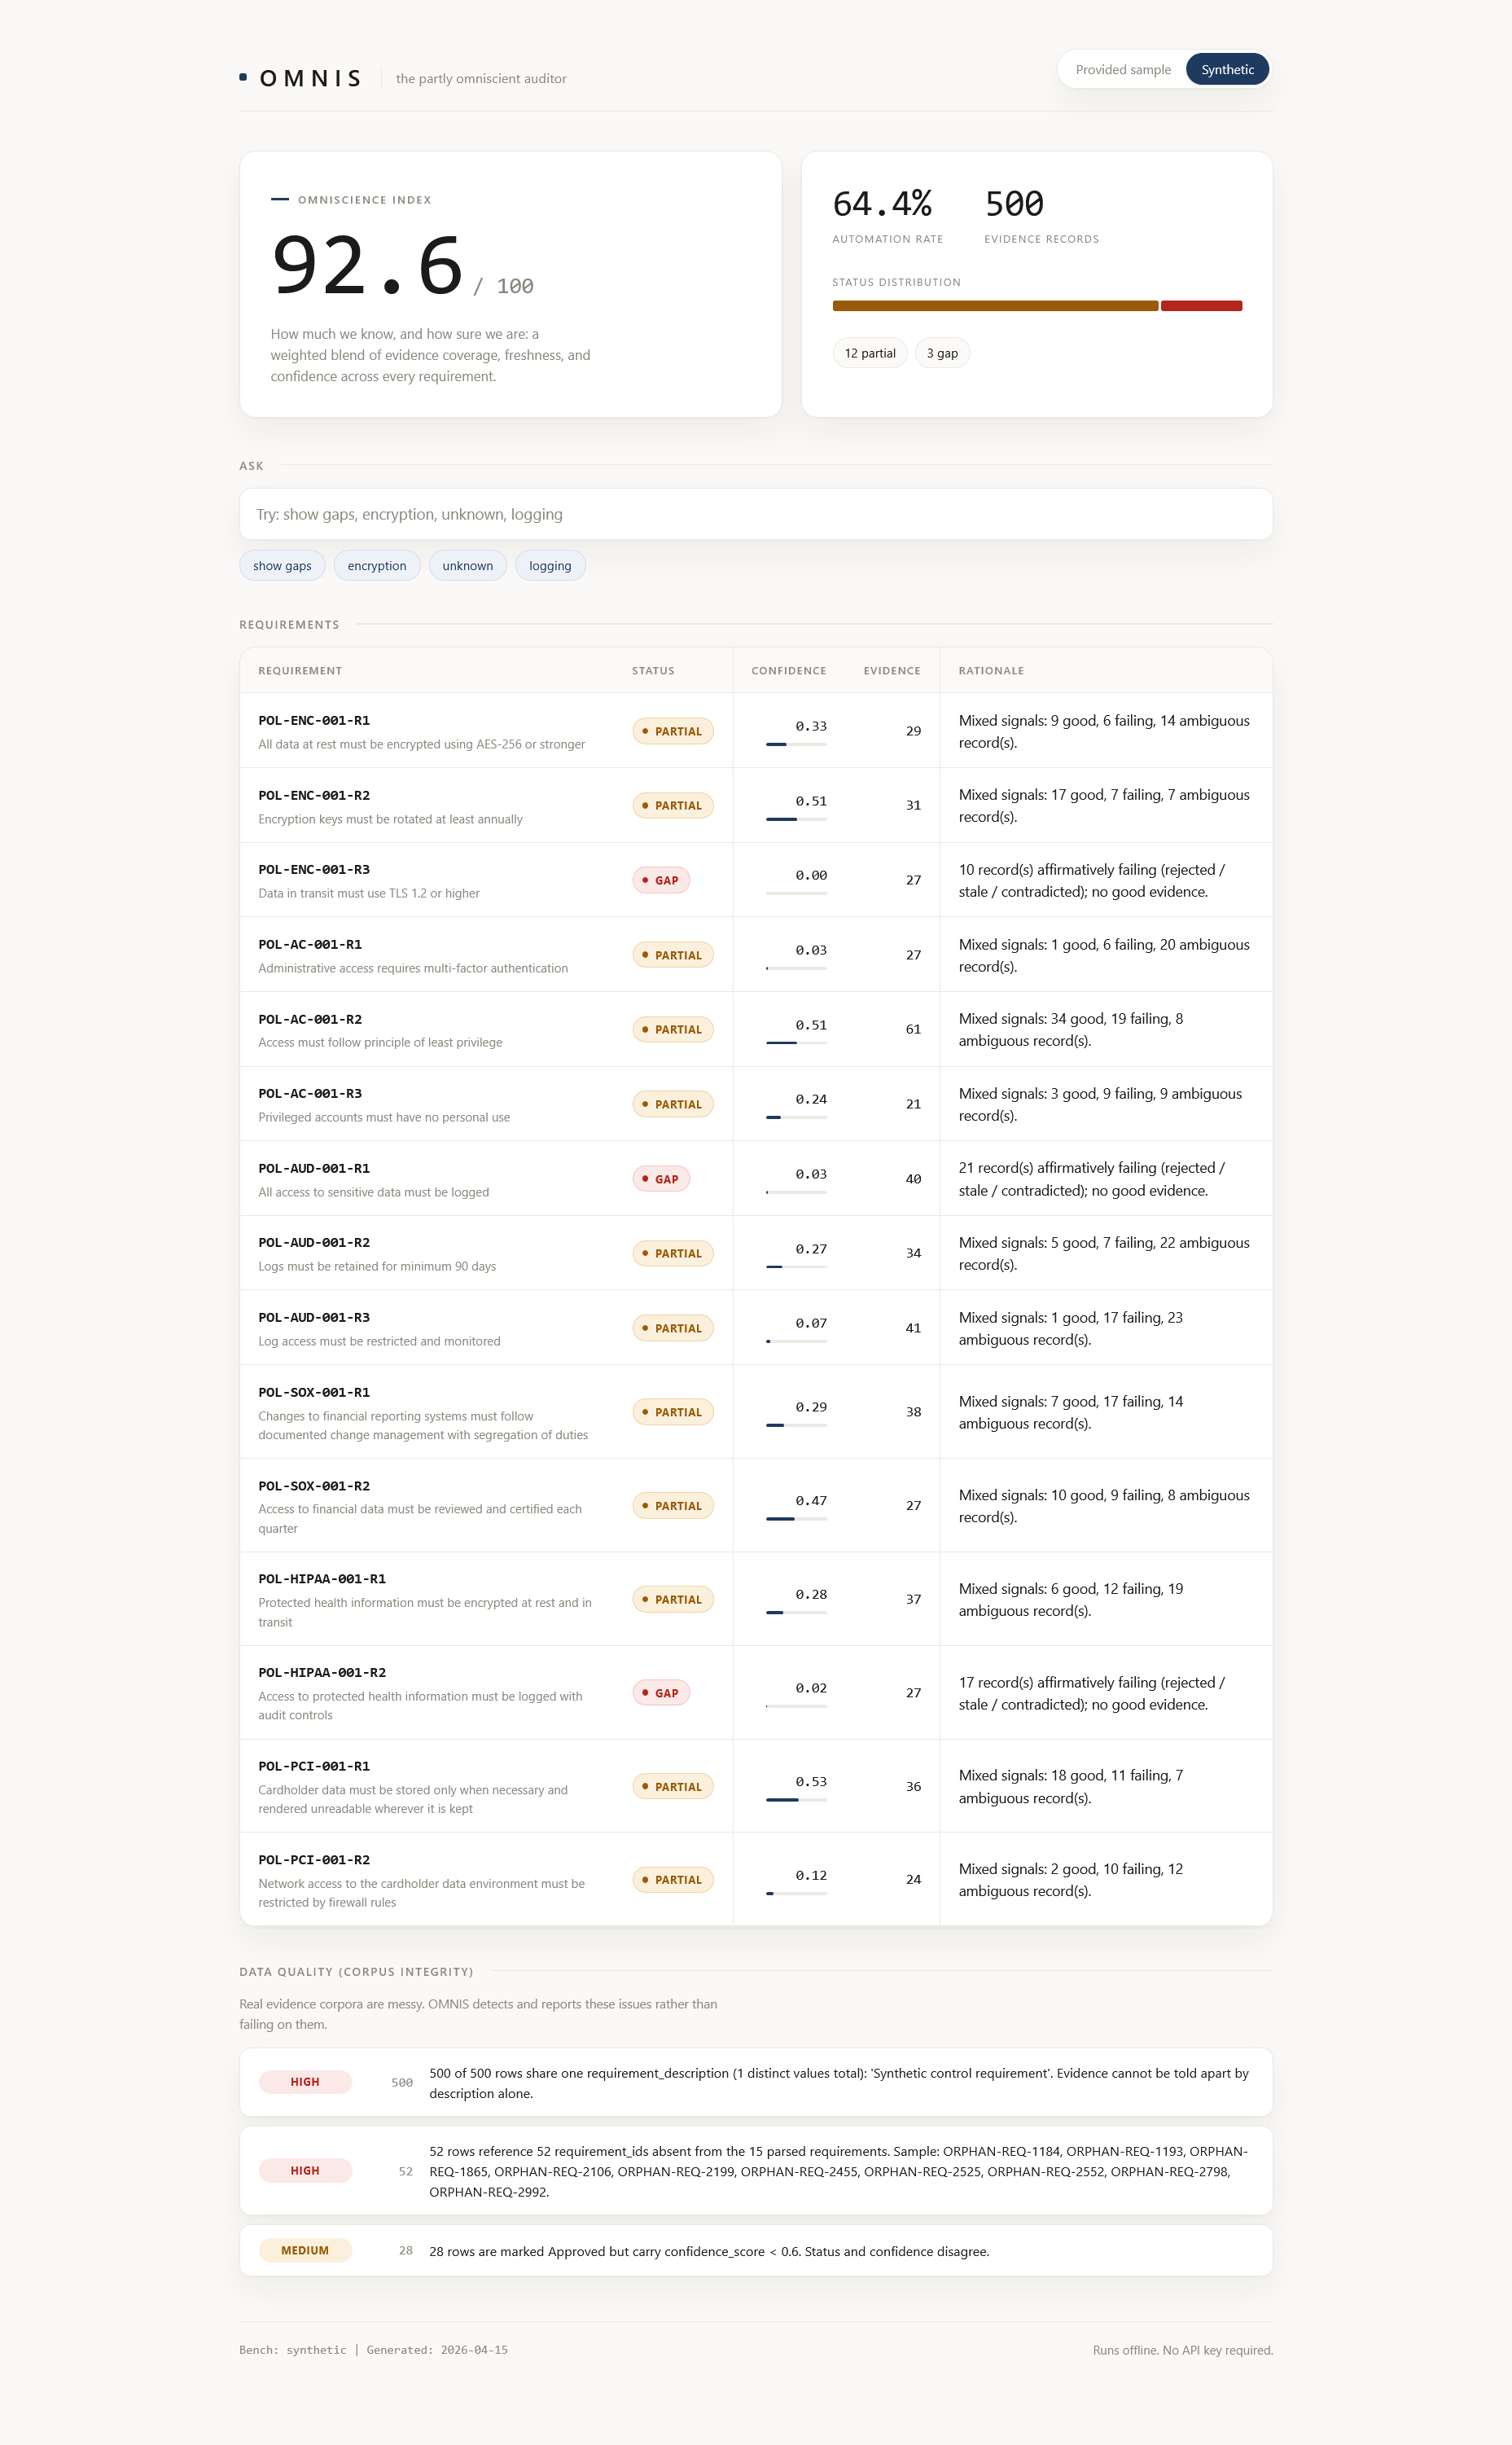
\includegraphics[width=0.6\linewidth]{hero.png}}
\caption{The single-page dashboard. Omniscience Index hero, automation rate, a status
distribution bar, the requirement table with status chips, and a data-quality panel. It
is one HTML file served by the Python standard library, no framework and no build step.}
\end{figure}

\begin{figure}[H]
\centering
\fbox{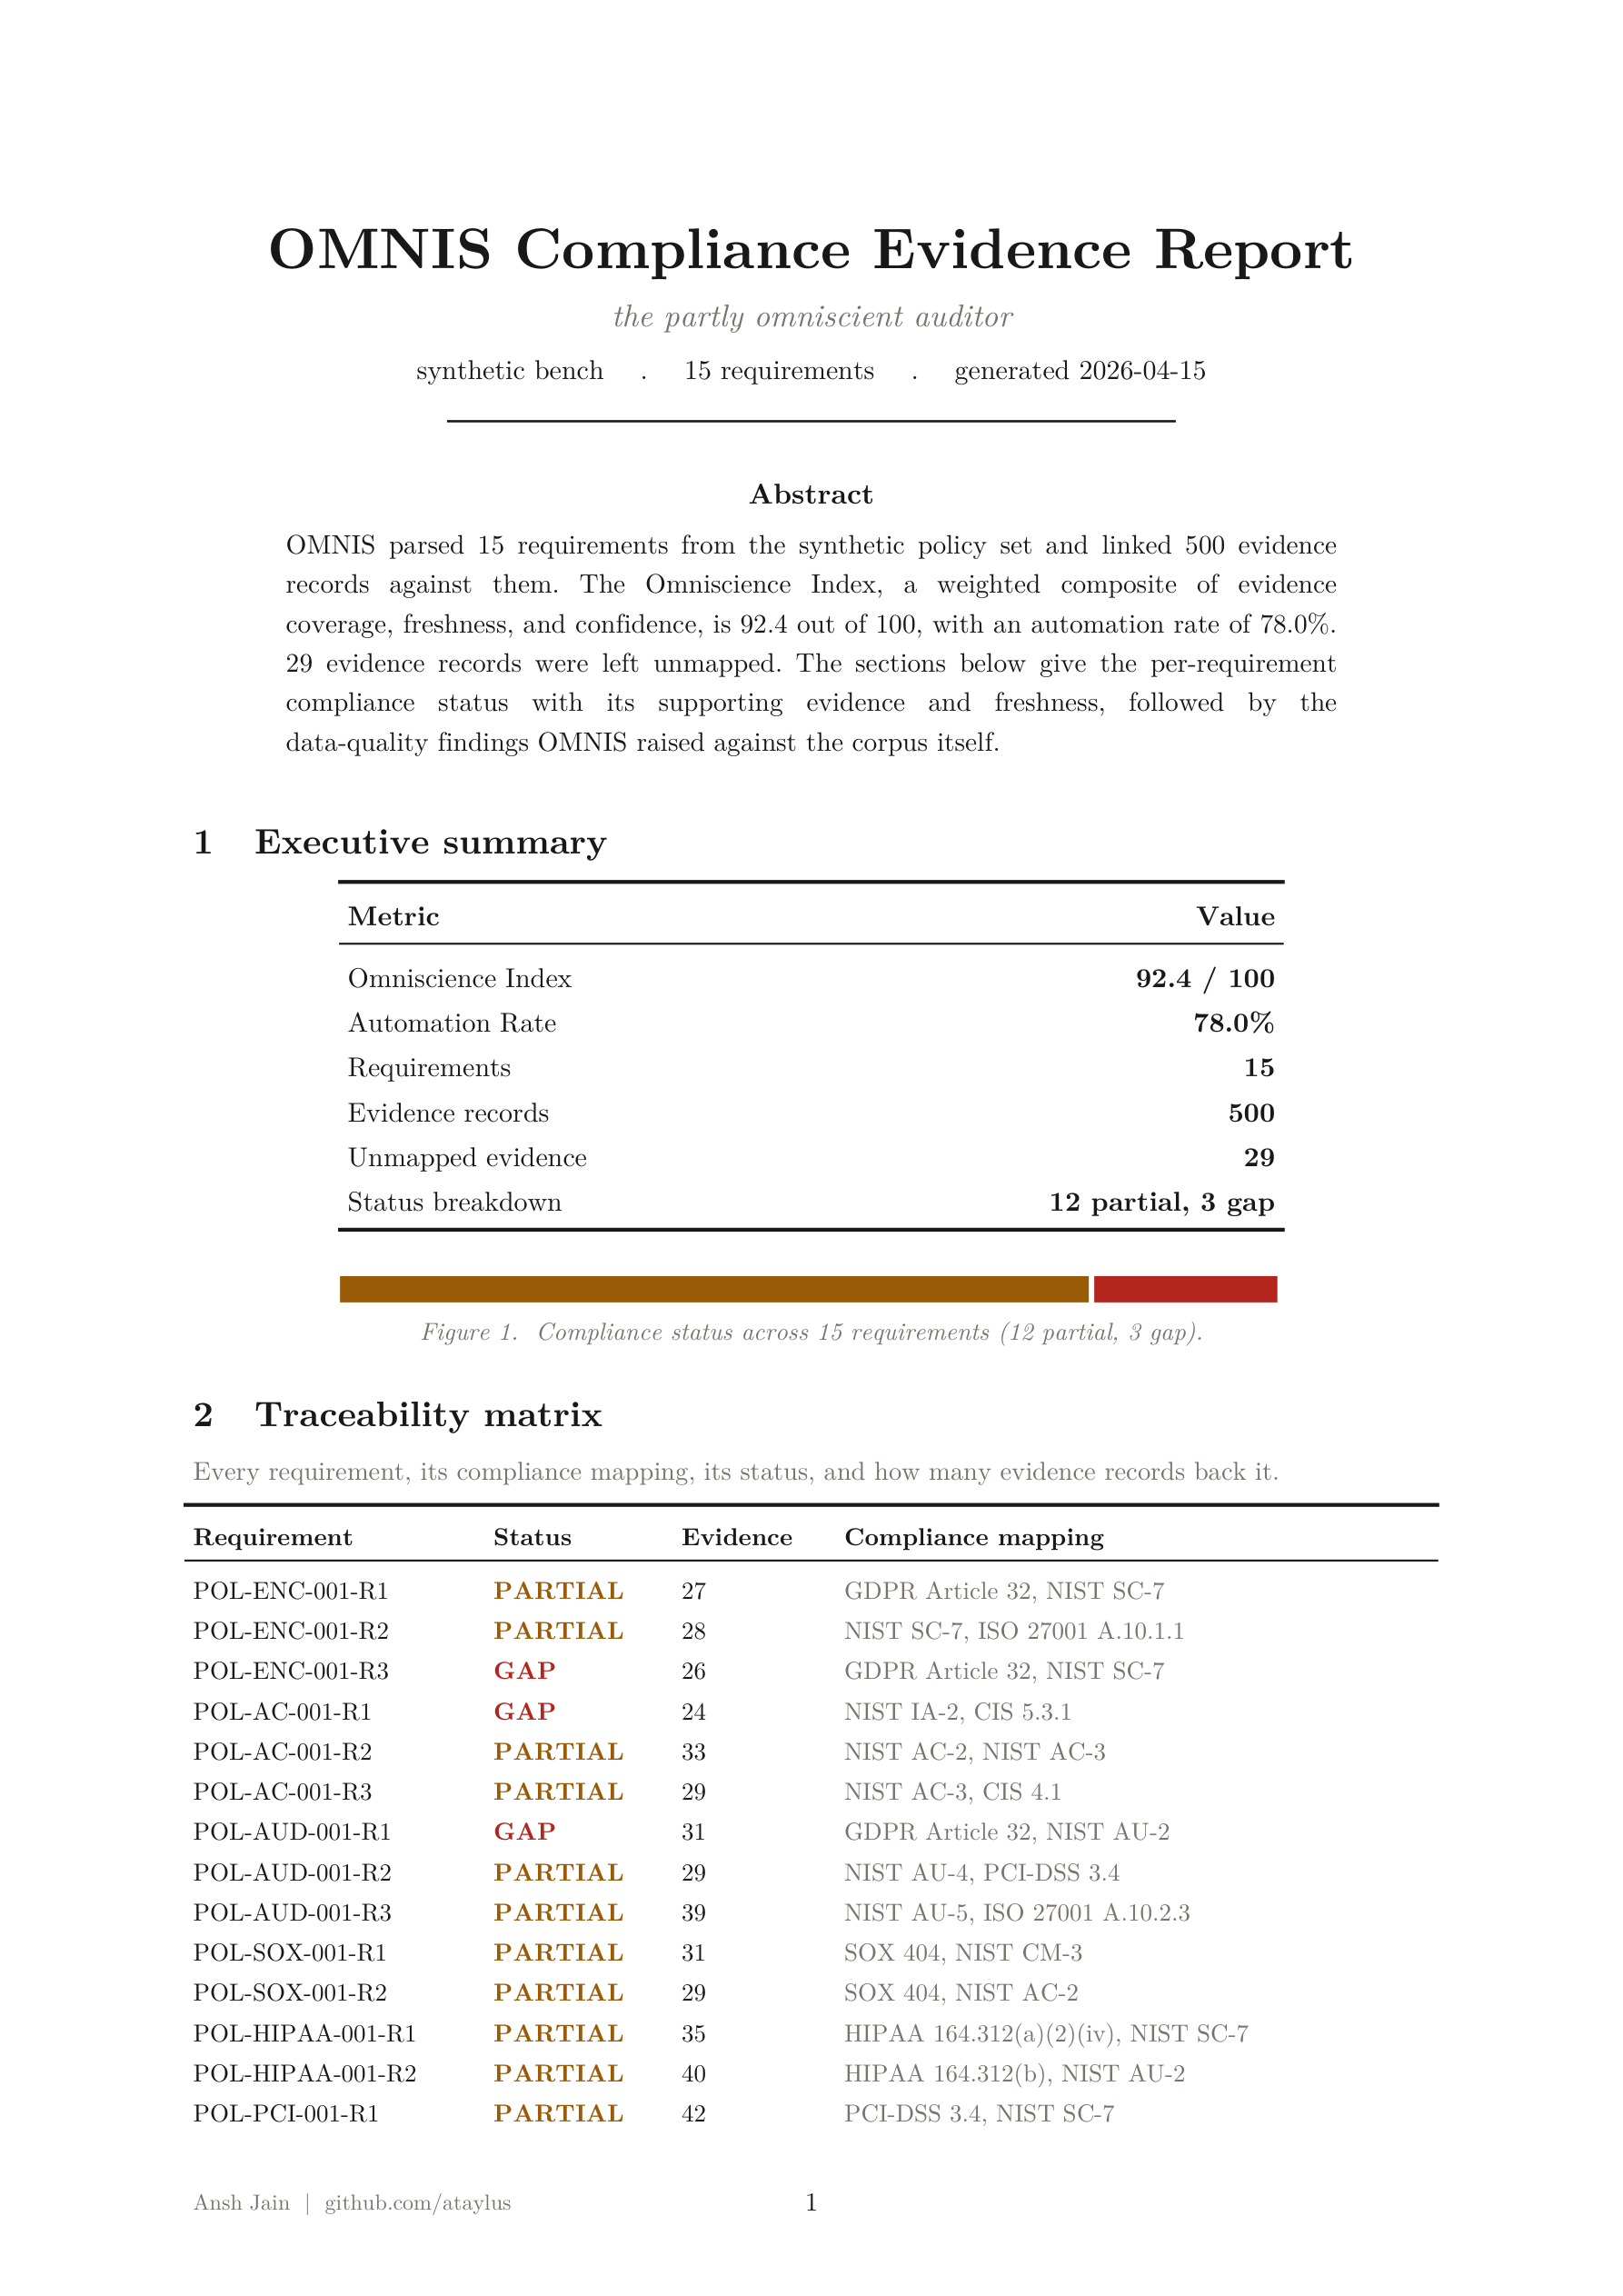
\includegraphics[width=0.45\linewidth]{fig_report_summary.png}}\hfill
\fbox{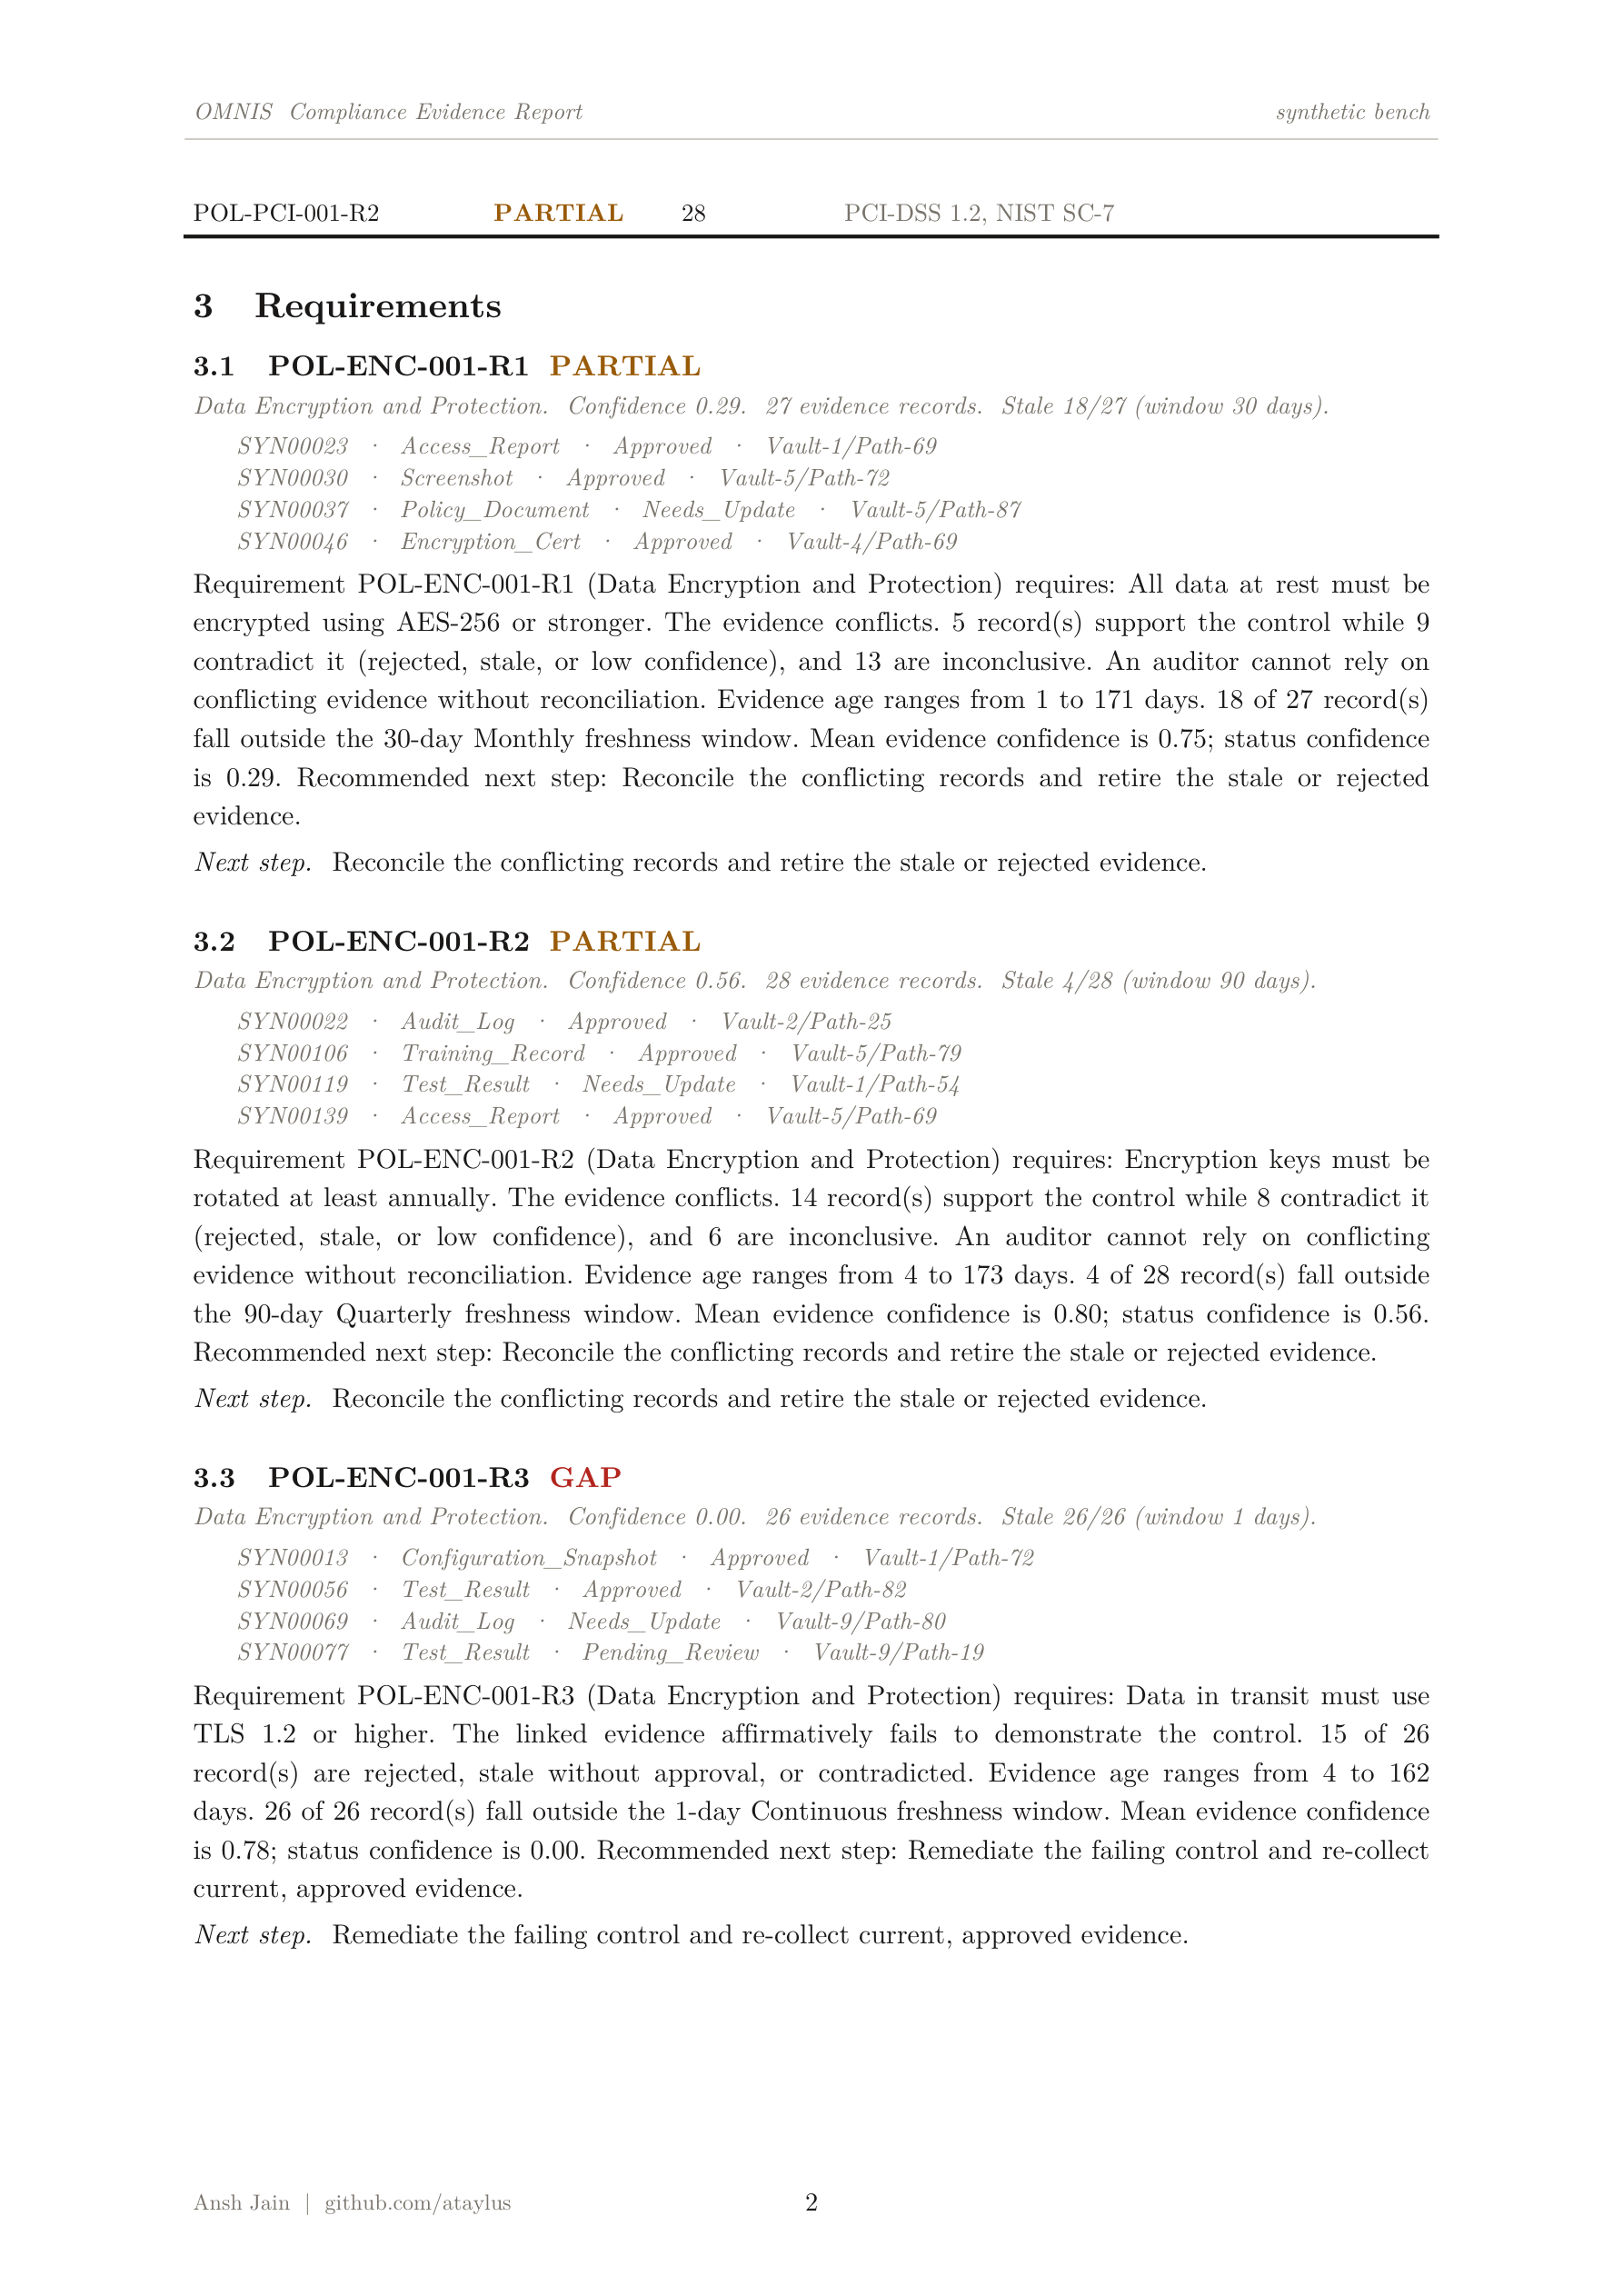
\includegraphics[width=0.45\linewidth]{fig_report_requirement.png}}
\caption{The auditor-ready report. A summary with the Omniscience Index, a traceability
matrix (requirement, status, evidence count, compliance mapping), then a section per
requirement with its linked evidence pointers and narrative, and an integrity appendix.}
\end{figure}

% ===========================================================================
\section{Design decisions}

The choices that shaped OMNIS, and the one-line reason behind each.

\begin{table}[H]
\sffamily\small
\renewcommand{\arraystretch}{1.3}
\begin{tabularx}{\linewidth}{@{}lX@{}}
\toprule
Decision & Why \\
\midrule
Deterministic parser first & Policy structure is structure; you parse it, you do not send it to a model and hope. \\
Layered linker, loud UNMAPPED & Cheap exact matches first, similarity only as a fallback, and an explicit unmapped verdict when nothing fits. \\
Rules before ML & A rule you can defend in a sentence beats an opaque model you cannot, especially once the provided labels turned out to be noise. \\
Recompute, do not trust & The stored freshness field is wrong on 455 of 500 rows, so freshness is recomputed from a fixed reference date, which also makes runs reproducible. \\
LLM off by default & The whole system runs on templates with no key, no network, and no cost. Live mode is wired and logs its own spend, but nothing depends on it. \\
Standard-library dashboard & One HTML file, no framework, no build step. It opens and works on a judge's laptop. \\
\bottomrule
\end{tabularx}
\caption{The decisions that shaped OMNIS, and the reasoning behind each.}
\end{table}

% ===========================================================================
\section{LLM policy and cost}

There is one LLM adapter, \code{omnis/llm.py}, with three modes. \textbf{off}, the shipped
default, returns nothing so every caller falls back to a deterministic template; the whole
system runs with no key, no network, and no cost. \textbf{cached} replays a recorded
response. \textbf{live} calls the API only if a key is present and logs every call with its
token estimate and cost. The performance numbers are measured with the LLM off; the model
never sits on the critical path.

Cost, as an estimate from the adapter's token heuristic and not a bill: a narrative
enrichment is about 400 input and 150 output tokens, roughly \$0.0012 per requirement,
about \$0.02 for all fifteen synthetic requirements and about \$0.58 even at the full
500-requirement scale. The real spend to date is \$0.00, because the system ships with the
LLM off.

% ===========================================================================
\section{Limitations}

Stated plainly. The two collectors are mock integrations: they read sample exports rather
than calling live APIs. The content linker is TF-IDF, a solid offline baseline rather than
semantic embeddings, so its exact-requirement recovery with the ID hidden is 54.7\%, well
above random but short of perfect. The synthetic bench is labelled by construction, which
is why the noisy provided sample remains the primary real-world test. Performance is
measured on a single laptop. None of these are hidden; each is reported where it is
relevant.

% ===========================================================================
\section{Reproducibility}

Everything runs offline on a clean machine:

\begin{quote}
\code{pip install -r requirements.txt}\\
\code{make demo} \quad opens the dashboard\\
\code{make test} \quad runs the 102 tests\\
\code{make analyze} \quad reproduces the label-independence finding\\
\code{python -m omnis report -{}-bench synthetic} \quad writes the report\\
\code{python -m omnis perf} \quad times 500 requirements + 5,000 evidence
\end{quote}

The full source, the committed report, and the analysis notebook are in the repository at
\url{https://github.com/ataylus/OMNIS}.

\vspace{1.4em}
{\color{line}\hrule height 0.5pt}
\vspace{0.5em}
\begin{center}
\sffamily\footnotesize\color{muted}
OMNIS, the partly omniscient auditor.\quad \watermark.\quad Team Partly Everything.
\end{center}

\end{document}
